In collaboration with several other institutions we have collected a dataset of diffractograms stemming from experiments, some of them labeled with corresponding structural information. The following paragraphs detail the contribution of each research group. Most data was collected using \ce{Cu} radiaton sources which have a  $K_{\alpha1}$ wavelength of $\lambda=1.54056\text{\AA}$ and a $K_{\alpha2}$ wavelength of $\lambda=1.54439\text{\AA}$. We filtered the submitted datasets to exclude patterns with invalid features such as the pattern containing only one unique recorded angle or negative angles, the pattern containing less than 50 recorded angles total, or all intensities being zero. The below Table$\eqref{tab:merged}$ provides an overview of the opXRD database. 

\begin{table}[!htb]
\centering
\caption{\footnotesize The opXRD database: The availability of the chemical composition, spacegroups, lattice parameters, and atomic coordinates of the underlying samples are indicated by the columns ``Comp.'', ``Spg.'', ``Lattice'' and ``Atom coords.'' respectively.}
\label{tab:merged}
\scalebox{0.79}{
\begin{adjustbox}{center}
\begin{tabular}{@{}lllllll@{}}
\toprule
\textbf{Institution} & \textbf{No. patterns} & \textbf{Comp.} & \textbf{Spg.} & \textbf{Lattice} & \textbf{Atom coords.} & \textbf{Research Project} \\
\midrule
CNRS        &  1052          & \cmark   & \partialcheck{85}   & \cmark   &  \partialcheck{85}   & Diffraction data extracted from the COD \\ 
HKUST(GZ)   &  21+499          & \cmark   & \cmark   & \cmark   & \cmark   & Phase/structure identification dataset  \\ 
USC         &  338          & \cmark   & \cmark   & \partialcheck{90}   & \xmark   & Study of CuNi and CuAl alloys          \\ 
EMPA        &  790          & \cmark   & \partialcheck{63}   & \xmark   & \xmark   & Tin halide perovskites, Zn-V-N libraries \\ 
INT         &  19,780        & \xmark   & \xmark   & \xmark   & \xmark   & Compilation of various projects        \\ 
IKFT        &  64           & \xmark   & \xmark   & \xmark   & \xmark   & Commercial catalysts, bulk materials   \\ 
LBNL        &  n/a          & \xmark   & \xmark   & \xmark   & \xmark   & Perovskites precursors, Mn-Sb-O system  \\ 
\bottomrule
\end{tabular}
\end{adjustbox}}
\end{table}

%TODO: A paragraph on how data is correlated
The degree of variation between the patterns is different for each contribution. For example, the CRNS and the INT contributions each are collections that encompass many research projects over a large period of time and hence exhibit a high degree of variability between individual patterns. In contrast, the contributions by the USC and the LBNL contain many very similar patterns. The patterns in the USC datasets are similar because the underlying samples are all variations of \ce{CuNi} and \ce{CuAl} alloys collected on the same machine. The patterns submitted by the LBNL are similar because they stem from in-situ recordings where several hundred or several thousand patterns were collected over time per sample while they were undergoing physical processes. 
\begin{figure}[!htb]
    \centering
    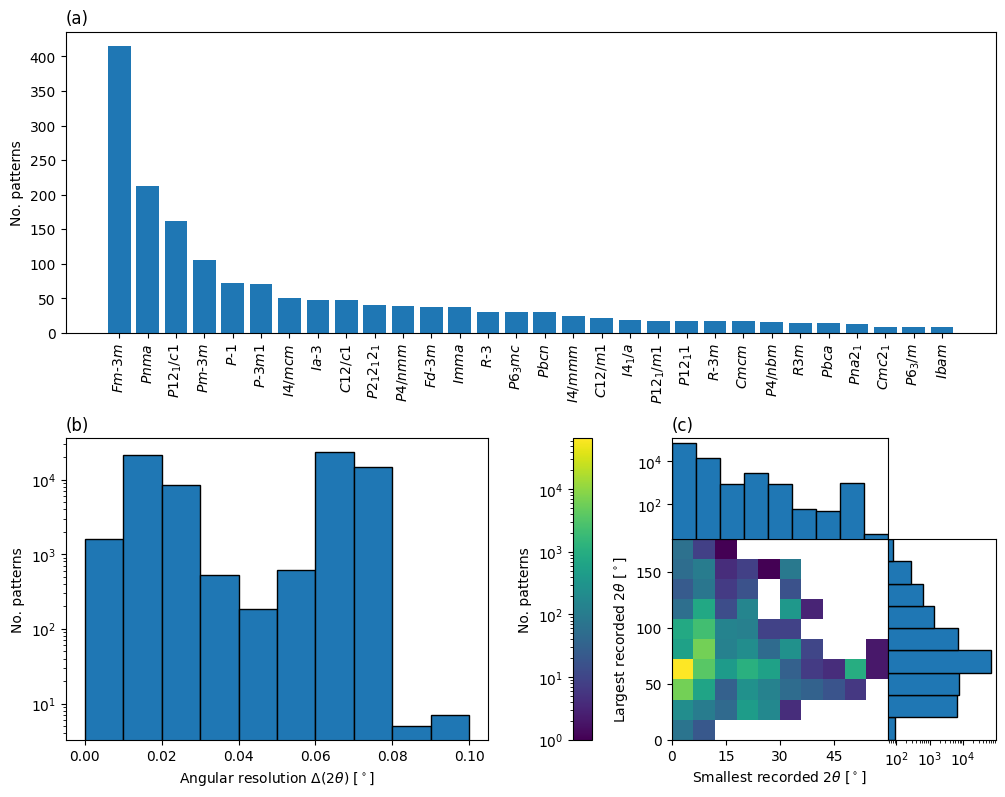
\includegraphics[width=0.8\linewidth]{figures/hist.png}
    \caption{Histograms detailing the distribution of properties in the opXRD dataset: a) distribution of spacegroups present in labeled data; b) distribution of angular resolution in all data; c) distribution of smallest and largest recorded $2\theta$ values for all data.}
    \label{fig:histograms}
\end{figure}


\pagebreak

%% Paragraph by FX Coudert and Arthur Hardiagon
\subsubsection*{Chimie ParisTech, PSL University}

Experimental pXRD data was extracted from the Crystallography Open Database (COD)\cite{Grazulis2009, Vaitkus2023}. The COD is, to our knowledge, the largest open-access collection of experimental crystal structures of organic, inorganic, and metal-organic compounds and minerals, containing more than 500,000 entries. The data in the COD are placed in the public domain and licensed under the CC0 License. Of the entire COD database 5432 structures contained at least one tag from the {CIF\_POW} dictionary, i.e., a tag relating to powder diffraction studies. These 5432 structures only account for 1\% of the total COD database, but this is to be expected since most crystal structures are resolved from single-crystal diffraction. Of these 5432 files, most contained only metadata related to the powder diffraction experiment, but did not include the raw data of the pattern itself. We could extract raw experimental pXRD patterns from 1052 files in total, after curation of a small number of files with clearly invalid data. \\

The pXRD data from the COD database are of high quality, with a median resolution of $\Delta(2\theta) = 0.013\degree$ and an average number of 9190 points measured per pattern. They span a wide chemical space, including organic, inorganic, and hybrid structures, and 75 different elements of the periodic table.

% Paragraph by Bin Cao and Tong-yi Zhang
\subsubsection*{Guangzhou Municipal Key Laboratory of Materials Informatics, HKUST(GZ)}

A small-scale experimental powder X-ray database called the X-Ray Phase Identification Public Experimental Dataset (XRed) was established over the past two years.\footnote{XRed can be accessed on GitHub at \url{https://github.com/WPEM/XRED}.} The primary objective of this database is to support the development of intelligent phase identification technology, serving as a foundation for data collection for future large-scale machine learning calculations. The XRed dataset primarily focuses on metal and metal-oxide particles, with data generated using instruments such as the Empyrean 3.0, Aeris, and Bruker D8 Advance diffractometers, all utilizing \ce{Cu} X-ray sources. Hundreds of pXRD patterns have been obtained through XRD refinement, enabling the determination of detailed lattice constants, atomic sizes, and other structural parameters. These patterns are labeled with CIF files that document the refined structures. The dataset is organized by elemental systems and includes original experimental files ranging from single-phase to five-phase mixtures, as well as mixtures studied for different tasks. \\

Another experimental dataset integrated with opXRD is a collection of powder diffraction data sourced from open-access publications and collaborating institutions. All collaborating institutions provided this data with full authorization for research purposes. This dataset provides broader coverage of chemical elements and includes ionic crystals, atomic crystals, and metallic crystals. This dataset surpasses Xred in size, containing 499 entries. However, contrary to Xred these data do not come paired with corresponding crystal structures.


Xqueryer,\footnote{Xqueryer can be accessed at \url{https://xqueryer.caobin.asia/}.} a recently launched cutting-edge free online platform for intelligent structure identification, will also serve as a source of data for the opXRD database. Users can upload experimental pXRD data to identify crystal structures and extract all relevant information available in the Materials Project database\cite{jain2013commentary}. Uploaded data are securely stored and integrated into the comprehensive opXRD database to progress toward a large-scale, long-term experimental resource. All usage complies with Xqueryer's terms of service.


% Paragraph by Adie Alwen and Andrea Hodge
\subsubsection*{Department of Chemical Engineering and Materials Science, USC}

Combinatorial \ce{CuNi} and \ce{CuAl} samples were synthesized at the University of Southern California (USC) via magnetron co-sputtering from \ce{Cu} (99.999\%) and \ce{Ni} (99.995\%) or \ce{Al} (99.999\%) targets (Plasmaterials) onto stationary $10 \si{cm}$ \ce{Si} (100) substrates yielding 169 unique $5 \times 5 \ \si{mm}$ squares per wafer. These alloys were selected to study compositional effects on stacking fault and growth twin boundary formation in sputtered materials \cite{alwen2024_1,alwen2024_2}. \\

XRD spectra were collected using a Malvern Panalytical Empyrean X-ray diffractometer at the Forschungszentrum Julich (FZJ) Institute for Energy and Climate Research, Structure and Function of Materials (IEK-2), which enabled automated XRD characterization due to its programmable XY stage and laser sensor for Z height correction. XRD analysis was used to link changes in defect formation in the sputtered films with varied phases and crystal structures. Each composition was characterized using \ce{Cu} $K_\alpha$ X-rays that were collimated to probe an area of $4 \times 4 \ \si{mm}$ using a step size of $0.026\degree$ and scan duration of $0.3$ seconds per step over a 2 range from $30\degree - 110\degree$. Measurement parameters were chosen to resolve at least six or more points above the full-width half maximum of each XRD peak.

% Paragraph by Alexander Wieczorek and Sebastiann Siol
\subsubsection*{Laboratory for Surface Science and Coating Technologies, Empa}

Combinatorial Zn–V–N libraries were synthesized using radio-frequency co-sputtering of Zn and V in a mixed Ar and \ce{N2} plasma. An orthogonal deposition temperature and composition gradient was created, resulting in a deposition temperature of $220\degree$C for samples 1~–~9 and $114\degree$C for samples 37~–~45. The composition for each sample was determined using X-ray fluorescence (XRF) spectroscopy which was further calibrated through Rutherford backscattering spectroscopy (RBS) based on selected samples. The newly identified and isolated semiconductor \ce{Zn2VN3} was identified to exhibit a cation-disordered wurtzite structure as verified by additional GI-XRD and SAED measurements\cite{Zhuk2021}. \\
Tin halide perovskites were deposited using single-step spin-coating as reported elsewhere\cite{Wieczorek2023}. Methylammonium lead iodide libraries with varying degrees of residual \ce{PbI2} were deposited using a two-step procedure involving both thermal evaporation of \ce{PbI2} and subsequent spin-coating of a methylammonium solution. The relative phase fractions were quantified using supplementary azimuthal angle scans coupled with structural factors and geometrical factors as reported elsewhere\cite{Wieczorek2024}. Fully inorganic lead perovskite libraries were prepared using thermal co-evaporation of lead and cesium halide salts. All metal halide perovskite libraries were measured within a custom-made X-Ray transparent inert-gas dome, resulting in the presence of minor additional features within the $\theta=19 \text{–}31\degree$ range. For all combinatorial libraries where any phases are specified, the complete set of phases is reported in the metadata. \\

XRD data was measured using a Bruker D8 Discover equipped with a Cu radiation source in a Bragg-Brentano geometry. For the reported data sets the instrument was equipped with a Goebel mirror effectively removing the Cu~K$\beta$ radiation. The data set originates from the combinatorial exploration of the Zn–V–N compositional space, as well as data gathered from multiple research activities on more established metal halide perovskite semiconductors. All data was collected from thin films deposited on borosilicate glass. The Zn–V–N films showed some preferential out-of-plane orientation, while for the perovskites the preferential orientation was minimal, resulting in the presence of all reflections. \\

%% Paragraph by Ben Breitung
\subsubsection*{Institute of Nanotechnology, KIT}

X-ray diffraction data was collected from a wide range of research projects conducted at the Institute of Nanotechnology over the past years. A major part of the research focused on high-entropy materials, which involved incorporating many different elements into single-phase structures, leading to peak shifts or phase separations. Most of those multi-component complex materials appeared in various structures, including rock-salt, spinel, fluorite, perovskite, and delafossite. The samples were prepared either in powder or in bulk form; therefore, powder XRD was performed on samples with adjusted height. The samples were prepared using various synthesis techniques, mostly solid-state or wet chemical syntheses, to obtain the desired structures. Consequently, particle size and crystallinity varied significantly. The sample set also includes samples that were not successfully measured or where phases could not be identified. \\

The X-ray diffraction data were collected on a Bruker D8 Advance using a Cu radiation source or a STOE Stadi P diffractometer equipped with a Ga-jet X-ray source. The samples were initially recorded for various research projects over the last ten years and were measured with different step sizes, times per step, and over different angle ranges, but all using \ce{Cu} $K_\alpha$ or \ce{Ga} $K_\beta$ radiation. The samples mostly contained transition metal oxides, sulfides, and fluorides. To improve statistics, the samples were rotated during the entire measurement. Some air-sensitive samples were measured using a transparent polymer dome for protection. This dome led to increased background noise over the first $20\degree$ and slightly decreased pattern resolution. \\ 

% Paragraph by Moritz Wolf 
\subsubsection*{Institute of Catalysis Research and Technology, KIT}

A variety of samples were analyzed including commercial catalysts, bulk reference materials, porous metal oxide particles, and nanoparticles. The latter were synthesized via the surfactant-free benzyl alcohol route \cite{Wolf2019, Wolf2018}. The cobalt oxide (\ce{CoO} or \ce{Co3O4}) and cerium oxide (\ce{CeO2}) nanoparticles were in the size range of $4-16 \ \si{nm}$ according to the Scherrer equation. A series of porous \ce{Al2O3} materials, which were prepared by calcination of boehmite (\ce{AlOOH}) at various temperatures, represents crystalline samples with limited long-range structure and various contributions of \ce{Al2O3} polymorphs. \\

X-ray diffraction (XRD) was conducted with an X’Pert Pro MPD (Panalytical) in Bragg-Brentano geometry using a \ce{Cu} X-ray source. The patterns were acquired in the $2\theta$ range of $5-80\degree$ with a step size of $0.016711\degree$ or $0.033420\degree$ and a total acquisition time of 40 to 120 min. This study has been carried out with the support of Angelina Barthelmeß, Elisabeth Herzinger, and Henning Hinrichs. \\

% Paragraph by Tim Kodalle
\subsubsection*{Molecular Foundry Division \& Advanced Light Source \& Chemical Sciences Division, LBNL}

In total three different datasets were collected. The first and second datasets focused on metal-halide perovskite precursor solutions. The first dataset was collected from spin-coating triple-cation metal-halide perovskite precursor solutions with the composition \ce{Cs}$_{0.05}$(MA$_{0.23}$FA$_{0.77}$)\ce{Pb}$_{1.1}$(\ce{I}$_{0.77}$\ce{Br}$_{0.23}$)$_{3}$ onto various substrates. Here, MA stands for Methylammonium and FA stands for Formamidinium. The substrates onto which these solutions were coated include glass, which is amorphous, and $\ce{GaAs}$ wafers, which are single crystalline. Other substrates were stacks of glass/indium tin oxide, stacks of \ce{GaAs}/CIGS, and stacks of glass/CIGS. Here, CIGS stands for a stack of \ce{Mo}, \ce{Cu}(\ce{In}, \ce{Ga})\ce{Se2},\ce{Cds} and \ce{ZnO}. Some of the substrates were additionally covered with a self-assembling monolayer of MeO-2PACz. The $\ce{GaAs}$ substrates were prepared by Dr. Jiro Nishinaga from the National Institute of Advanced Industrial Science and Technology (AIST) in Japan and the glass/CIGS substrates by Dr. Christian Kaufmann and his team at Helmholtz-Zentrum Berlin (HZB) in Germany. Data collection was performed in situ during thin-film deposition using a custom-made spin-coating and annealing stage. \\

A second dataset was collected from spin-coating metal-halide perovskite precursor solutions with varying compositions of \ce{MAPb(I_{1-x}Br_x)3} spin-coated onto glass substrates. Here, MA = Methylammonium and x = 0, 0.33, 0.5, 0.67, 1. The substrates were preheated to different temperatures including $30\degree $C, $50\degree $C, $70\degree $C, and $90\degree $C, and the spin-coating process was performed at a constant temperature on the preheated substrates. For both datasets, diffraction data were continuously measured during spin-coating, chemical induction of crystallization, and annealing of the samples, at $100\degree$C and $110\degree$C respectively. The diffraction data was recorded with a frequency of about $0.56 
 \ 1/\si{s}$ and $0.54 \ 1/\si{s}$. Each in situ measurement consisted of about 500 to 1000 individual diffractograms. Depending on the substrate, each series of diffractograms shows an evolution from substrate only to a combination of polycrystalline perovskite, $\ce{PbI2}$ and substrate via several intermediate phases. \\

For these two datasets, experimental XRD data were collected at beamline 12.3.2 of the Advanced Light Source, the synchrotron at Lawrence Berkeley National Laboratory. The data were collected using a photon energy of 10 $\si{keV}$ ($\lambda = 1.23984 \text{\AA}$), selected using a Si(111) monochromator. Measurements were taken in grazing incidence geometry, i.e. using a beam incidence angle of $1\degree$. Two-dimensional diffraction images were recorded using a Dectris Pilatus 1M area detector at an angle between $34\degree$ and $36\degree$ with a sample-to-detector distance of roughly $190 \ \si{mm}$. The two-dimensional data were calibrated using an Al$_{2}$O$_{3}$ calibration standard and integrated along the azimuthal angle. \\

% Paragraph by Gregoire Heymans

A third dataset was collected by observing the phase evolution of an Mn-Sb-O system with varying annealing temperatures. The temperatures used to analyze the crystal structure of the Mn-Sb-O system were chosen depending on the number of phase transitions appearing for a certain temperature range. Few changes in the crystal structure appear between room temperature and 300$\degree$C and phase transitions appeared from 300$\degree$C until 850$\degree$C. No phase transition appeared when cooling down. Therefore, the crystal structure was measured every 100$\degree$C between room temperature and 300$\degree$C; every 50$\degree$C between 300$\degree$C and 850$\degree$C; and every 200$\degree$C when cooling down. The heating and cooling rates are fixed for all the experiments at 50$\degree$C/min and the holding time is fixed at 2 min. \\

The data was collected using the \textit{in situ}  Rigaku-SmartLab3kW diffractometer. This tool operates with SmartLab Studio II software, which can measure the X-ray diffraction during the annealing process. This enables directly showing all the phase transitions when annealing in various atmospheres such as \ce{O2}, \ce{Ar}, and \ce{NH3}. Phase transitions are analyzed with the \textit{in situ} XRD tool up to 850$\degree$C in this work. Most of the \textit{in situ} experiments were performed under an air-like 20\% \ce{O2} and 80\% \ce{Ar} environment is chosen (\ce{Ar} flow: 50 \si{sccm}, \ce{O2} flow: 10 \si{sccm}). When a 100\% Ar environment is fixed, an Ar flow of 60 \si{sccm} is input. The Bragg-Brentano (BB) mode is preferred in terms of geometry because it is more adapted in the analysis of scarce phases such as  \ce{MnSb2O6} rutile. The angular step used in the recording was 0.01$\degree$ and the scanning rate was 10$\degree$/min. 

% end of Gregoire Heymans



